% TEMPLATE for Usenix papers, specifically to meet requirements of
%  USENIX '05
% originally a template for producing IEEE-format articles using LaTeX.
%   written by Matthew Ward, CS Department, Worcester Polytechnic Institute.
% adapted by David Beazley for his excellent SWIG paper in Proceedings,
%   Tcl 96
% turned into a smartass generic template by De Clarke, with thanks to
%   both the above pioneers
% use at your own risk.  Complaints to /dev/null.
% make it two column with no page numbering, default is 10 point

% Munged by Fred Douglis <douglis@research.att.com> 10/97 to separate
% the .sty file from the LaTeX source template, so that people can
% more easily include the .sty file into an existing document.  Also
% changed to more closely follow the style guidelines as represented
% by the Word sample file. 

% Note that since 2010, USENIX does not require endnotes. If you want
% foot of page notes, don't include the endnotes package in the 
% usepackage command, below.

% This version uses the latex2e styles, not the very ancient 2.09 stuff.
\documentclass[letterpaper,twocolumn,10pt]{article}
\usepackage{usenix,graphicx,epstopdf,endnotes,subfigure, url}

\bibliographystyle{acm}

\usepackage{listings}
\lstset{basicstyle=\ttfamily\footnotesize,
    frame=single,
    breaklines=true
}

\begin{document}

%don't want date printed
\date{}

%make title bold and 14 pt font (Latex default is non-bold, 16 pt)
\title{\Large \bf Evaluation of SciDB for Image and Video Processing Tasks}

%for single author (just remove % characters)
\author{
{\rm Mohammed Suhail Rehman \qquad Advisor: Kayvon Fatahalian}\\
School of Computer Science\\
Carnegie Mellon University
} % end author

\maketitle

% Use the following at camera-ready time to suppress page numbers.
% Comment it out when you first submit the paper for review.
\thispagestyle{empty}


\subsection*{Abstract}
In this report, we evaluate the use of SciDB, an array database, for image processing workloads. We explore the representation of images in SciDB, select four specific image-processing tasks to implement in SciDB, and evaluated them on an AWS cluster using a dataset of a 1000 high-resolution images. Even with a simple and non-optimized MPI baseline, we find SciDB to be an order of magnitude slower. We conclude this report by analysing our observations and propose future work that may improve SciDB's feasibility for such workloads.

\section{Introduction}


SciDB\cite{stonebraker2013scidb} is a computational DBMS designed to cater to the data storage needs of the scientific community. SciDB envisions to bring the convenience and performance of database management systems to the scientific community for large-scale computational workloads.

SciDB is designed to be multi-dimensional, with an array-based data model. It also provides support for data versioning and provenance which is a oft-cited feature requirement of data management systems from scientists.
 
SciDB has been used in various scientific domains, including geo-spatial data, genomics\cite{stonebraker2011architecture} as well as astronomy\cite{Cudre-Mauroux:2009:DSS:1687553.1687584}.

On paper, SciDB's array-based data model seems to align with how images are digitally represented. Thus, we were interested in investigating the use of SciDB for Image processing workloads. Through our work, we want to answer the following questions:

\begin{itemize}
\item Can we represent and store images, videos, and image patches\footnote{An image patch is a small square region (also known as a tile) of an image} efficiently in SciDB?
\item Can image processing tasks be expressed in the form of database queries on images stored within SciDB?
\item What is the performance of the proposed SciDB based solution 
on a suite of simple image/video analysis tasks vs. a comparable distributed implementation of the same tasks?
\end{itemize}

As a stretch goal, we further wanted to evaluate the possibility of integrating existing deep network evaluation systems with SciDB storage via SciDB's UDF mechanisms. However, given our experiences with SciDB's performance in all of our initial benchmarks, we focused on optimizing the basic image processing tasks and were unable explore the use of SciDB for deep network evaluation. The interested reader will be referred to one such attempt, discussed in the related work section (\S \ref{sec:relwork}) of this report.

The rest of the report is organized as follows: \S\ref{sec:motivation} talks about the motivation of this work, followed by the related work in \S\ref{sec:relwork}. We then discuss the project implementation in \S\ref{sec:implementation}, starting with the representation of images in SciDB in \S\ref{sec:images}, followed by the description of the individual image processing tasks in \S\ref{sec:tasks}. Our evaluation platform and methodology is discussed in \S\ref{sec:eval}, followed by the results and analysis in \S\ref{sec:results}. Finally, we summarize our contributions in \S\ref{sec:future} and discuss the implications for future work.

\section{Motivation}\label{sec:motivation}
Image processing finds importance in various fields: from search, to robotics, to next-generation mobile applications. With the advent of smart phones and other devices, the amount of user-generated images and video generated daily is only exploding. 

Large-scale image processing is being used for projects such as 3D world reconstruction from photos and live, interactive, virtual reality video. As a result, systems need to process streams of images and video and be able to store and retrieve them in increasingly efficient ways.

Array databases such as SciDB offer the ability to store large volumes of multidimensional data and perform computation on the data in the form of database queries. One can envision a SciDB-based image retrieval solution that automatically performs the required computation to answer queries such as ``\texttt{Select all images which average intensity greater than some threshold}'', or using higher-order features such as ``\texttt{Select all videos containing Cats}''. For this to happen, we must be able to assess the ability of such systems to perform the required computation for image and video processing. In this work, we explore the ways in which images can be represented in SciDB and how low-level image processing operations can be expressed in the form of database queries.

\section{Related Work}\label{sec:relwork}

\subsection{Image Storage and Retrieval}
Image and video retrieval systems have been of major interest over several decades; many approaches have been discussed and studied. {\em Concept-based image retrieval systems}, (also known as {\em description-based} \cite{ASI:ASI1153} systems) use auxiliary information and meta-data (such as image descriptive tags, image dimensions, EXIF and geo-location tags) to index images; although this approach is used to supplant systems such as web-based image/video search, its ability to locate and retrieve images and/or video is limited to the quality of information that is supplied in context or in the meta-data.

On the other-hand, there has been a lot of attention paid to {\em content-based image retrieval systems} (CBIR), which use image processing and classification methods to automatically classify and index images. There are many approaches in this domain, an exhaustive list is beyond the scope of this report; interested readers may refer to a fairly recent survey by Datta et. al \cite{Datta:2008} for details. Traditional methods involved the extraction of low-level features, such as edges, color and texture in images, and the use of distance measures (such as Euclidean or Cosine) to rank image search results and narrow down candidate images for retrieval.

The accuracy of these traditional methods have been surpassed by machine-learning-based approaches, most notably, deep learning\cite{Wan:2014}. Unlike conventional machine learning methods that often use only a few stages of learning, deep learning mimics the human brain; the processing is organized in a deep architecture and passes information through multiple stages of transformation and representation. By exploring deep architectures to learn features at multiple levels of abstraction in an automated fashion, deep learning methods allow a system to learn complex functions that directly map raw sensory input data to the output, without relying on human-crafted features.

Among various deep learning approaches, the {\em Convolutional Neural Network} (or CNN / ConvNet) approach for deep learning has recently surpassed all known methods for large-scale visual recognition, and have been adopted for use in commercial systems by Google, Facebook and Baidu.  Multiple open-source deep-learning frameworks based on CNNs have emerged, such as \cite{cudaconvnet, icml2014c1_donahue14, DBLP:journals/corr/SermanetEZMFL13}. However, they have been surpassed in terms of features, performance and popularity by the Caffe system\cite{Jia:2014}, which I intend to study and use for this capstone project. Caffe currently uses Google's Protocol Buffers\cite{protobuf} to store Models and LevelDB\cite{levelDB} to store training and input data. Caffe has been designed to support multiple CPUs or GPUs in a shared memory context, no efficient distributed implementations of Caffe currently exist to my knowledge.  

\subsection{Scale-out Approaches to Image Storage and Retrieval} \label{bigdata}

The methods discussed in the previous section with regards to content-based image retrieval (CBIR) are largely designed for execution in shared-memory systems or systems with GPU-accelerated support. In this section, we will review some of the research efforts into scale-out approaches for image storage, processing and retrieval systems.

\textbf{Image Storage}: The rise in popularity of cloud-based object storage systems such as Amazon's S3\cite{S3} has become a boon for web application developers looking for a scalable solution for BLOB storage. Similarly, a number of highly-distributed image storage systems have been built using a distributed architecture such as Twitter's Blobstore\cite{blobstore} and Facebook's Haystack\cite{beaver2010finding} and f4\cite{f4}. These systems rely on external databases to keep track of image metadata and are simple image storage and serving systems. They are optimized to serve content to millions of users while optimizing throughput and latency, and are incapable of performing non-trivial image processing tasks on the images stored in the systems. 

\textbf {Scale-out CBIR and Machine Learning}: The research regarding the feasibility of cluster-based distributed CBIR implementations, mostly using the Message-Passing Interface (MPI) framework is sparse, interested readers are directed to \cite{1508203} for an example. Renewed interest in cluster-based CBIR emerged with the rise in popularity of Hadoop MapReduce \cite{premchaiswadi2013improving, gu2012content, 6632112}. 

Distributed frameworks for machine learning are aplenty, a example system based on Hadoop is Mahout\cite{owen2011mahout}. GraphLab\cite{low2012distributed} is a distributed framework designed specifically for iterative graph-based computation, which can be applied for certain types of machine learning systems. A fairly recent technique for scaling out machine learning computation is based on the concept of a parameter server\cite{Li:2014:SDM:2685048.2685095}, a high performance distributed key-value that is used to store model parameters for machines that are working in parallel to train and use machine learning models. CloudCV\cite{DBLP:journals/corr/AgrawalMGCBMOB15} is distributed image processing framework that uses a number of underlying distributed systems including GraphLab. StormCV\cite{stormCV} enables the use of Apache Storm for video processing by adding computer vision (CV) specific operations to Apache Storm\cite{storm}.

For deep learning, Chilimbi et. al.\cite{chilimbi2014project} describe the design and implementation of a scalable framework called Project Adam, which relies on data serving machines providing training inputs to model training machines that asynchronously update a shared model via a global parameter server. The authors evaluated Project Adam's performance using 120 cluster nodes for image classification - this work presents a promising baseline to compare our proposed system against.  


\subsection{Array and Computational Databases}
For my work, I intend to explore the use of multi-dimensional array databases for a variety of image processing tasks, including CBIR. In this section, I will discuss the history and evolution of array databases.

The limitations of the relational database model with regards to multi-dimensional data was understood early on\cite{baumann}; the ANSI/ISO SQL standard\cite{ISO:SQL} supports only one-dimensional arrays. Array data such as Images can be stored in relational databases using {\em binary large object} types (BLOBs), but have many disadvantages - BLOB data fields typically have poor performance as modern SQL engines are not optimized for storage and retrieval of large binary objects. More importantly, BLOBs cannot be effectively used in a query, users can simply store, retrieve or possibly query the size of BLOBs but cannot make queries against its content. 

Modern web-based frameworks such as Django \cite{django} rely on a two-tiered approach to storing images: Image information and metadata that is required for the application is stored in a traditional database, which typically contains a location path (file or URL) that can be used to retrieve the actual binary contents of the image. As discussed in \S\ref{bigdata}, several internet-scale companies have built special-purpose distributed storage systems to support high-throughput, low-latency storage and retrieval of BLOBs. 

Early work describing multi-dimensional, array-style databases was first stipulated by Baumann\cite{baumann}. Libkin et. al.\cite{Libkin:1996} formulated a calculus for arrays and implemented a query language that specifically targets multi-dimensional arrays. Further work in the domain resulted in the creation of the Raster Data Manager (RasDaMan) system\cite{Baumann:1998,Rasdaman}. RasDaMan has been in active development since 1998 and is the longest-running array database project.  

Commercial projects in the 90s and 2000s that involved the storage of multi-dimensional data was driven by the lucrative Geographic Information Systems (GIS) market. Oracle GeoRaster\cite{oracle}, TerraLib\cite{camara2008terralib} and PostGIS\cite{obe2011postgis} are examples. More recently, databases that support the nested data model as part of the Data Definition Language (DDL), such as MongoDB are being increasingly used in web-based applications that interact with map data provided by public map APIs such as Google Maps and OpenStreetMap.

SciDB\cite{stonebraker2013scidb} is a computational array DBMS designed to cater to the data storage needs of the scientific community. SciDB is designed to be multi-dimensional, with an array-based data model. It also provides support for data versioning and provenance which is a oft-cited feature requirement of data management systems from scientists. SciDB differs from the previous related work in its focus on computation - SciDB intends to push computation to the data by supporting queries that can perform some type of computation on the stored arrays, similar to RasDaMan. However, RasDaMan uses Postgres in the back-end for blob storage, while SciDB is built from ground-up to support efficient storage and retrieval of array data in a scale-out environment. Although the newest of all the work described in this section, SciDB has already been used in various scientific domains, including geo-spatial data, genomics\cite{stonebraker2011architecture} as well as astronomy\cite{Cudre-Mauroux:2009:DSS:1687553.1687584}. 

To my knowledge, no known framework or system has explored the use of array databases for CBIR, however some work exists that is similar in flavor. Planthaber et. al. \cite{planthaber2012earthdb} describe the use of SciDB to process and store NASA's  Moderate Resolution Imaging Spectroradiometer (MODIS) data on a SciDB cluster. Using SciDB, they have demonstrated the ability to write fairly simple queries that generate a composite RGB image from the MODIS data by selecting the appropriate spectral bands (one for each color channel), within specific geographic coordinates; a second workload they demonstrate is the use of the red and near-infrared spectral bands to compute the presence of vegetation (known as the Normalized Difference Vegetation Index (NDVI)). In \cite{Moyers:2013:DIP:2536274.2536306}, Moyers e.t al. describe the AscotDB, a web-based tool that enables the collaborative analysis of telescope images and metadata. AscotDB uses SciDB for array processing; iterative-processing features were added to SciDB to support this specific use-case.

\section{Implementation}\label{sec:implementation}

\subsection{SciDB Architecture and Array Model}\label{sec:arch}

\subsubsection{SciDB Architecture}
SciDB uses a shared-nothing architecture which is shown in Figure \ref{fig:arch} below.

\begin{figure*}[ht]
\centering
\includegraphics[width=.6\textwidth]{figures/scidb_architecture.eps}
\caption{SciDB Cluster Architecture}
\label{fig:arch}
\end{figure*}


SciDB is deployed on a cluster of servers, each with processing, memory, and local storage, interconnected using a standard Ethernet and TCP/IP network. Each physical server hosts a SciDB instance that is responsible for local storage and processing.  A PostgreSQL database is used to store the SciDB catalog of array schema and the distribution of data in the cluster.

External applications, when they connect to a SciDB database, connect to one of the instances in the cluster. While all instances in the SciDB cluster participate in query execution and data storage, one server is the coordinator and orchestrates query execution and result fetching. It is the responsibility of the coordinator instance to mediate all communication between the SciDB external client and the entire SciDB database. The rest of the system instances are referred to as worker instances and work on behalf of the coordinator for query processing.

For testing and evaluation purposes, SciDB also works on a single physical machine in a ``pseudo-distributed fashion'', with multiple SciDB engines spawned on a single physical machine.

\subsection{The SciDB Data Model - Arrays}
SciDB arrays are expressed in terms of two basic parameters:  the {\em dimensions} of the array, as well as {\em attributes} of the array. 

\subsubsection{Array Dimensions}
An n-dimensional SciDB array has dimensions ($d_{1}$, $d_{2}$,$...$,$d_{n}$). The {\em size} of each dimension is the number of ordered values in that dimension. For example, a 2-dimensional array may have dimensions $i$ and $j$, each with values $(1, 2, 3, ..., 10)$ and $(1, 2, ..., 30)$ respectively. SciDB uses 64-bit integers to represent the values in each dimension, but also support non-integer dimensions such as variable-length strings or floating point integers. Furthermore, SciDB supports the notion of dimensional bounds. When the total value of a dimension is known in advance, the array can be declared with a {\em bounded} dimension. Sometimes, the cardinality of the array may not be known at array creation time. In such cases, the array can be declared with an {\em unbounded} dimension. It must be noted, however, that certain array operations are restricted to arrays with integer bounded dimensions.

In addition to the dimension size attributes, the user must define two parameters for each dimension: the {\em chunk size} and {\em chunk overlap} parameters. These parameters affect the distribution of the array data among the worker nodes and need to be studied with respect to their effect on the performance of the image operations that we intend to deploy in SciDB.

\subsubsection{Array Attributes}
An n dimensional array in SciDB refers to a single cell or element of an array. However, each array in the SciDB array can hold multiple data values known as {\em attributes}. Each data value is referred to as an {\em attribute}, and can be any of the supported data types in SciDB.

Therefore, during the creation of an array in SciDB (analogous to the declaration of a table schema in a relational database), the user must specify:

\begin{itemize}
\item An array name - a simple string which can be used to refer to the array in all operations involving the array.
\item The dimensions of the array. The name and size of each dimension must be declared, with the exception of unbounded dimensions, whose size is represented using the asterisk character (\texttt{*}).
\item At least one attribute for the array. Attributes can be added to an array as the result of an operation in SciDB.
\end{itemize}

An example of an array definition in SciDB is given below:

\begin{lstlisting}[caption=Creating an Array in SciDB, frame=single]
AQL% CREATE ARRAY open <val:double>[I=0:9,10,0,J=0:*,10,0];
\end{lstlisting}

In the example, the name of the array is \texttt{open}, with one attribute named \texttt{val}, of type \texttt{double}. This array consists of two dimensions, \texttt{I} and \texttt{J}. \texttt{I} is a bounded dimension with values ranging from 0 to 9, with chunk size 10 and chunk overlap 0. \texttt{J} another dimension similar to \texttt{I}, but the size of this dimension is unbounded.

\subsection{Query Languages and Array Operations}
SciDB currently supports two distinct query languages: the {\em Array Query Language} (AQL) the and {\em Array Functional Language} (AFL). AQL is very similar to SQL, where operations are described as \texttt {SELECTS, INSERT, UPDATE} with support for various types of \texttt{JOINS}. On the other hand, AFL allows for a more functional description of array operations, using a function syntax which allows for nesting of operations. AFL has a few advantages over AQL in terms of the verbosity of queries, however, from my initial work with SciDB I believe that the query languages do not intersect perfectly in terms of the operations supported; some operations may only be performed in AQL (such as joins along a dimension), while some others can only be performed in AFL. 

SciDB is designed to perform a number of operations on Arrays. An extensive listing of array operations is beyond the scope of this document, the interested reader is referred to the SciDB manual\cite{SciDBManual}. However, the operations that can be performed on an array can be broadly classified into the following: array selection, array operations (such as cross product, joins etc.), aggregation operations (which can return either arrays or scalars) and so on.

\subsection{Representing Images in SciDB}\label{sec:images}
Images can be represented in multiple ways, and this has an effect on the type and performance of image array operations that are performed in SciDB.

\subsubsection{Loading Image Data and Conversion to SciDB Arrays}
SciDB allows multiple client types to interact with the database (see \S\ref{sec:arch}).  For this project, I chose the SciDB-py client interface to python\cite{SciDBPy}. This interface allows for SciDB arrays to be accessed and manipulated using python variable bindings. In addition, it supports the conversion of SciDB arrays to and from numpy arrays. This is useful since the scikit-image library\cite{van2014scikit} in python allows for the reading of various image file formats and loading of the pixel data into numpy arrays. 

\subsubsection{Representing a single image in SciDB}\label{sec:singleimage}
An image can be considered to be an array of intensity values for each pixel in an image. A single image can be represented in SciDB in a number of ways:

\begin{itemize}
\item A 3-dimensional array consisting of a single attribute: intensity. The dimensions are image width, height and color channel (such as red, green and blue (RGB)) The array schema for this representation (assuming an image has 480x320 pixels) is represented in listing \ref{imgarray} 

\begin{lstlisting} [caption=A 3-dimensional Image Array in SciDB, frame=single, label=imgarray]
<f0:uint8> 
[width=0:479,1000,0, 
height= 0:319,1000,0, 
channel=0:2,1000,0]
\end{lstlisting}

\item A 2-dimensional array with 3 attributes, one attribute per channel.
\end{itemize}

\subsubsection{Representing Multiple Images in SciDB}
It follows from the previous discussion that there are again many ways in which multiple images can be represented in SciDB. This design decision influences the way in which queries are constructed for the image processing operations. We have identified two specific ways in which multiple images can be represented in SciDB (Figure \ref{fig:arrays}):

\textbf{Individual Arrays}: Each image can be represented as an individual array in SciDB using the methods described in \S\ref{sec:singleimage}. One drawback of this method is that the operations that involve multiple images require array joins, as will be described in \S\ref{sec:tasks}.

\textbf{Volume of Images}: Multiple images can be encapsulated as a single array of multiple images with an extra dimension that represents an index to an image (see Listing \ref{imgsarray}). In this approach, multiple images can be ``flattened'' into a single image using aggregation for the image operations that we explore in \S\ref{sec:tasks}. This approach is great for images that have the same dimension (such as individual frames for a video). SciDB also has support for sparse arrays and unbounded dimensions and it remains to be seen if the approaches that discuss in \S\ref{sec:tasks} are applicable for spare and/or arrays with unbounded dimensions.

\begin{lstlisting} [caption=A 4-dimensional image volume in SciDB, frame=single, label=imgsarray]
<f0:uint8> 
[width=0:479,1000,0, 
height= 0:319,1000,0, 
channel=0:2,1000,0,
image=0:*,1,0]
\end{lstlisting}



\begin{figure}[htp]
\centering
	\subfigure[Images stored as individual arrays in SciDB]{\includegraphics[width=0.25\textwidth]{figures/array1.eps}}
    \subfigure[Images stored as a volume in a single array in SciDB]{\includegraphics[width=0.15\textwidth]{figures/array2.eps}}
	\caption{Ways to represent Images in SciDB}
	\label{fig:arrays}
\end{figure}



\subsection{Image Processing Benchmarks}\label{sec:tasks}
We plan to develop queries sec:WIAorm the following fundamental image primitives in SciDB. For each operation that we discuss in this section, we have to develop the equivalent SciDB expressions to perform the image operation and evaluate their performance. The image processing benchmarks that have been constructed are:

\begin{itemize}
\item Weighted Image Average (\textbf{WIA})
\item Image Patch Extraction and Average (\textbf{IPE})
\item Convolution (\textbf{CONV})
\item All Pairs Nearest Neighbours (\textbf{APNN})
\end{itemize} 

\subsubsection{Weighted Image Average} \label{sec:WIA}
In this operation, a collection of related images are combined to produce a single image using some kind of average. The specific variant we look at in this study is the weighted average of a volume of images.

As an example, the queries required to average N individual arrays is presented in  program listing \ref{avg1}. This operation requires a cross-join between each individual array and the target array in an iterative fashion, followed by a sum of the individual elements. Each element of the resulting array is then divided (scalar division) to produce the final average image.

\begin{lstlisting}[caption=Averaging N individual image arrays in SciDB, frame=single, label=avg1]
store(project(apply(join(sum,image), y, sum.x + image.x), y), sum)
store(project(apply(sum, z, sum.x / n ), z), sum)
\end{lstlisting}

The weighted image averaging operation (as presented in listing \ref{avg2}) when applied to a volume of images can be expressed as three separate operations: A dimension join to associate each individual image in the volume with the associated weight of the image, an aggregation operation where each element of each image is multiplied with its associated weight and then flattened, and finally a scalar division operation to divide each element of the resulting image with the sum of weights to produce the final, weighted average image.

\begin{lstlisting}[caption=Weighted Average of images in a single SciDB Volume, frame=single, label=avg2, float]
SELECT * INTO temp_average FROM average_img JOIN weights ON average_img.i3 = weights.i0;
store(aggregate(apply(temp_average,weighted_image,f0*weight),sum(weighted_image),i0,i1,i2),average_image);
store(project(apply(average_image,weighted_image_avg, weighted_image_sum / $WEIGHTTOTAL ),weighted_image_avg),average_image2)
\end{lstlisting}

\subsubsection{Image Patch Extraction and Average} \label{sec:IPE}
The IPE benchmark consists extracting a square patch (also known as tile) portion of the image volume from each image to construct a new image volume of patches. This volume is then averaged using the weighted image average query described in \S\ref{sec:WIA}. This operation can be done in two distinct ways:

\begin{itemize}
\item Extract patches from each image using a fixed coordinate for the patch location, as illustrated in Figure \ref{fig:patch1}. 

\item Extract the patches from each image at variable locations, as illustrated in Figure \ref{fig:patch2}. This is a more complex query, which requires iterating over the image array for each image and extracting the required subregion of the image and adding it to the patch volume.
\end{itemize}


\begin{figure*}[htp]
\centering
	\subfigure[Extracting image patches from a fixed region on each image]{\label{fig:patch1}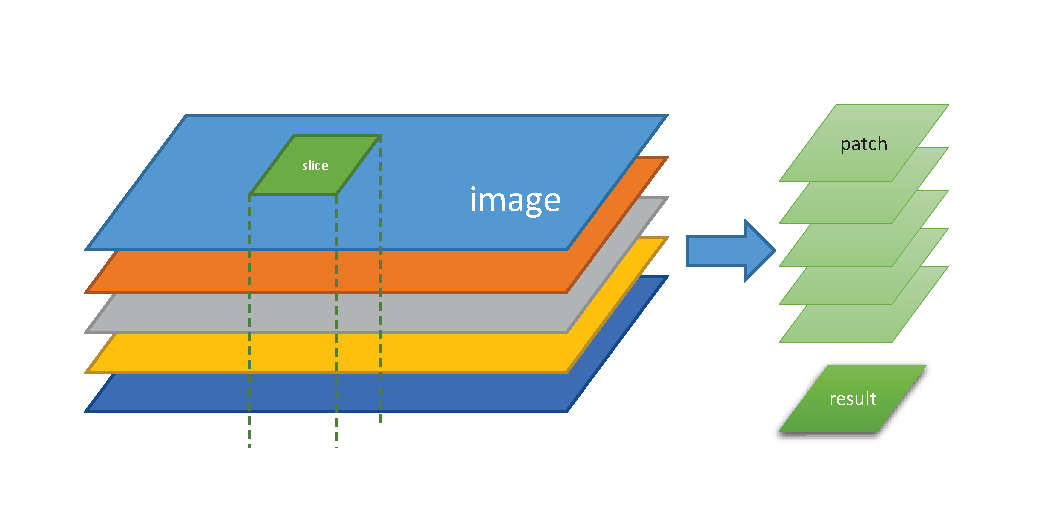
\includegraphics[width=0.35\textwidth]{figures/patch1.eps}} \hspace{1 em}
    \subfigure[Extracting image patches from a variable region on each image]{\label{fig:patch2}\includegraphics[width=0.35\textwidth]{figures/patch2.eps}}
	\caption{Patch extraction implementations for our study}
	\label{fig:patch}
\end{figure*}


\subsubsection{Fixed Patch Location Implementation}
Extraction of patches from a fixed region in each image is fairly straight-forward in SciDB. The \texttt{subarray()} function allows for a fixed region of an array to be extracted from the volume of images. Once the patches have been extracted and stored as a single volume of patches, the average patch image can be computed using the same algorithm described in \S \ref{sec:WIA}. The exact query used for this operation is provided in Listing \ref{lst:IPE1}.

\begin{lstlisting}[caption=Fixed Image Patch Extraction, frame=single, label=lst:IPE1, float]
aggregate(apply(cross_join(subarray(image_volume,$PATCH_X_START,$PATCH_Y_START,0,0,$PATCH_X_END,$PATCH_Y_END,2,$NUM_FILES) as patch_volume, weights,patch_volume.i3,weights.i0),weighted_image,f0*weight),sum(weighted_image),i0,i1,i2);
\end{lstlisting}

\subsubsection{Variable Patch Location Implementation}
To extract patches from different coordinates for each image in a volume of images, a single DB query can not longer be used. Instead, we have to iterate over each image in the volume, and slice out the image patch. The patch is appended into the the volume of patches. Once the patches have been extracted and stored as a single volume of patches, the average patch image can be computed using the algorithm described in \S \ref{sec:WIA}.


\subsubsection{Convolution} \label{sec:CONV}

The convolution operation on an image involves the calculation of each pixel value as being some kind of weighted aggregate of itself and its neighbouring pixel values. The weights are specified as a convolution {\em kernel}. Convolution is illustrated in Figure \ref{fig:convo}. Different convolution kernels result in different output images being generated, aggregations generally result in image smoothing, while special kernels with negative weights at certain neighbouring pixels can be used to highlight the edges in an image. 

\begin{figure}[h]
\centering
\includegraphics[width=.4\textwidth]{convolution.png}
\caption{Convolution Operation on an Image using a convolution kernel\protect\footnotemark}
\label{fig:convo}
\end{figure}

\footnotetext{Image Source: \url{https://developer.apple.com/library/ios/documentation/Performance/Conceptual/vImage/Art/kernel_convolution.jpg}}

While SciDB does not explicitly support convolution with arbitrary kernels, it support windowed aggregation using the \texttt{window()} function. This allows the values within an $N$-dimensional neighbourhood of an array element to be aggregated using some aggregation function, such as \texttt{sum()} or even a user-defined aggregation function. Image convolution using specific kernels, such as the box-blur kernel can be  performed in SciDB by using a \texttt{3x3} window over each image plane and using the \texttt{sum()} aggregation function.

\subsubsection{All-Pairs Nearest Neighbours} \label{sec:APNN}
The APNN benchmark for a given image dataset involves the calculation of a distance matrix and computing the k Nearest Neighbours for every image represented in the distance matrix. Typically, this is computed using higher-order features, but for this benchmark, we will use the sum of squared distance between each pair of pixels as the distance function for two images. 

In SciDB, the operations involved in the APNN benchmark are illustrated in figure \ref{fig:apnn_scidb}. First, a cross-join of the image volume is performed with itself across the image dimension to produce all pairs of pixel values. Next, the sum of square distances is computed using the \texttt{apply()} and \texttt{aggregate()} functions to produce a distance matrix for all pairs of images. Finally, a special kNN function that computes the ranks of image similarities can be computed. 

\begin{figure*}[ht]
\centering
\includegraphics[width=\textwidth]{figures/scidb_apnn.eps}
\caption{All Pairs Nearest Neighbors in SciDB}
\label{fig:apnn_scidb}
\end{figure*}

\section{Evaluation Methodology and Experimental Setup}\label{sec:eval}
For each of the image operations discussed in \S\ref{sec:tasks}, we produce different sequence of queries in SciDB that achieve the intended image processing operation. These can be compared to a baseline implementation in MPI.

\subsection{Image Datasets}
We plan to use a number of datasets that can be used to evaluate the performance of our SciDB image processing operations. All the operations described in \S\ref{sec:tasks} are low-level pixel operations that are not dependent on the actual content of the images, we can use any collection of images, while varying image resolution to assess the performance impact of small images versus larger images. For our experiments, we went with a common video resolution of $1920x1080$. In the case of APNN, due to the sheer volume of data generated by the cross join as illustrated in Figure \ref{fig:apnn}, we restricted the SciDB experiments to 64x64 thumbnails obtained from the MIRFLICKR thumbnail dataset\cite{huiskes08}. A Large number of image frames of the same resolution, channels and bit depth can be easily generated from videos. For this experiment we generated the 1080p video frames from Big Buck Bunny \cite{BBB}, an open-source 3D animated short film, available under a creative commons license. 



\subsection{Baseline MPI Implementations}
In order to perform a baseline comparison of SciDB's performance for these types of image processing tasks, we implemented the same algorithms using the Message Passing Interface (MPI) framework. In this model, we assumed a shared storage model for input and each MPI process can independently access each and every image file in the dataset. In general, we had two types MPI program flows for the baseline implementations:


\begin{figure*}[ht]
\centering
	\subfigure[Map, Gather \& Reduce flow for  the WIA, IPE and APNN benchmarks]{\label{fig:mpi1}\includegraphics[width=0.35\textwidth]{figures/mpi1.eps}} \hspace{1 em}
    \subfigure[Map-only program flow for the Convolution (CONV) benchmark]{\label{fig:mpi2}\includegraphics[width=0.35\textwidth]{figures/mpi2.eps}}
	\caption{Baseline MPI Implementations}
	\label{fig:mpi}
\end{figure*}

\textbf{Map, Gather, Reduce}: This flow consists of a map-style phase where each processor independently processes image files that are assigned to it, produces an intermediate result that is then gathered on the master process and finally reduced to the final output. Represented in Figure \ref{fig:mpi1}, this flow was used to implement the baseline MPI version for the WIA, IPE and APNN benchmarks. 

\textbf{Map only}: This flow consists of a map-style phase where each processor independently processes image files that are assigned to it,  and produces an output file that is written independently to the shared disk. Represented in Figure \ref{fig:mpi2}, this flow was used to implement the baseline MPI version for the convolution (CONV) benchmark. 

\subsection{Cluster Configuration}
Part of our study requires us to explore the performance of these image processing applications on a virtual cluster deployed on AWS. For this, we have devised an cluster configuration that suits both the use of SciDB as well as MPI. Figure \ref{fig:cluster} illustrates our cluster configuration while Table \ref{tab:config} contains the configuration of the individual nodes. Each node has a single attached SSD-based instance store of 32 GB which is used by SciDB as the Database store and scratch space. In addition, a single EBS volume is exported using NFS to all the nodes in the cluster, allowing for the input dataset to be accessible to all of the nodes via NFS.


\begin{figure}[h]
\centering
\includegraphics[width=.45\textwidth]{figures/scidb_cluster.eps}
\caption{Cluster Layout}
\label{fig:cluster}
\end{figure}

\begin{table} \label{tab:config}
\begin{tabular}{|l|p{3cm}|}
\hline
\textbf{Category} & \textbf{Configuration}  \\
\hline
Instance Type     & \texttt{m3.large}                                                        \\
Virtual CPUs      & 2 vCPUs from Intel Xeon E5-2670 (Ivy or Sandy Bridge) \\
RAM               & 7.5 GB                                                          \\
Root EBS Volume   & 25 GB                                                           \\
Instance Storage  & 32 GB SSD \\
\hline
\end{tabular}
\end{table}

\section{Results}\label{sec:results}
In this section, we describe a few performance results obtained in implementing SciDB and comparing the performance of SciDB against a few baselines. First, we present a few results of tests performed during the implementation of these image processing operations on a laptop. We then scale up to a cluster on AWS with 16 nodes.

\subsection{Single-Machine Experiments}
All of the results presented in this section are from running SciDB on a laptop with Core i7 and 8GB of Memory. Even though SciDB was running on a single machine, it was configured to launch 4 instances of the database nodes.

\subsubsection{Weighted Image Average}
The first experiment was to ascertain the performance of WIA using either images in individual arrays or an array of images as a single image volume. As discussed in the system design diagram, we can represent a set of images in individual arrays or as a volume of images as shown in Figure \ref{fig:arrays}. 

To evaluate the difference in the approaches, we show run an experiment to show the time taken to average $N$ small (64x64) images, where $N = \{10,100,1000\}$. The results are presented in Figure \ref{fig:avg_result}.

Performing the image averaging operation across $N$ individual arrays requires a cross-join between each individual array and the result array in an iterative fashion, followed by a sum of the individual elements. Each element of the resulting array is then divided by $N$ (scalar division) to produce the final average image. The performance of this approach is in Figure \ref{fig:avg_result}, represented as the series \texttt{Averaging N Arrays}.

\begin{figure}[h]
\centering
\includegraphics[width=.55\textwidth]{figures/wia_single.eps}
\caption{Single Machine Image Averaging Time}
\label{fig:avg_result}
\end{figure}

A marked improvement is noticed when the $N$ images are combined into a single array, effectively containing a volume of images. The performance of this approach is in Figure \ref{fig:avg_result}, represented as the series \texttt{Weighted Volume Average}. In this case, Image averaging is expressed as three separate operations: A dimension join to associate each individual image in the volume with the respective weight of the image, an aggregation operation where each element of each image is multiplied with its associated weight and then flattened, and finally a scalar division operation to divide each element of the resulting image with the sum of weights to produce the Final, weighted average image.  Although this operation performs more work than the queries used to average N arrays, it performs an order of magnitude faster. 

Notice however, that in spite of the improved performance of SciDB using the image volume approach, it is still many orders of magnitude slower than a simple in-memory calculation of the average image using a simple C program that sequentially iterates over each pixel, adding up the pixel values for each image, represented as the series \texttt{Native Program} in Figure \ref{fig:avg_result}.

Given that storing $N$ images as a single ``image volume'' array is significantly faster for this simple task than storing them as separate arrays, we will continue using this volume of images approach as the image representation in SciDB for the remaining experiments.

\subsubsection{Image Patch Extraction}
For the IPE benchmark, we wanted to see the difference in runtime for the two approaches for IPE explained in \S\ref{sec:IPE}. The two different techniques are compared in Figure \ref{fig:patch_result}. 

\begin{figure}[h]
\centering
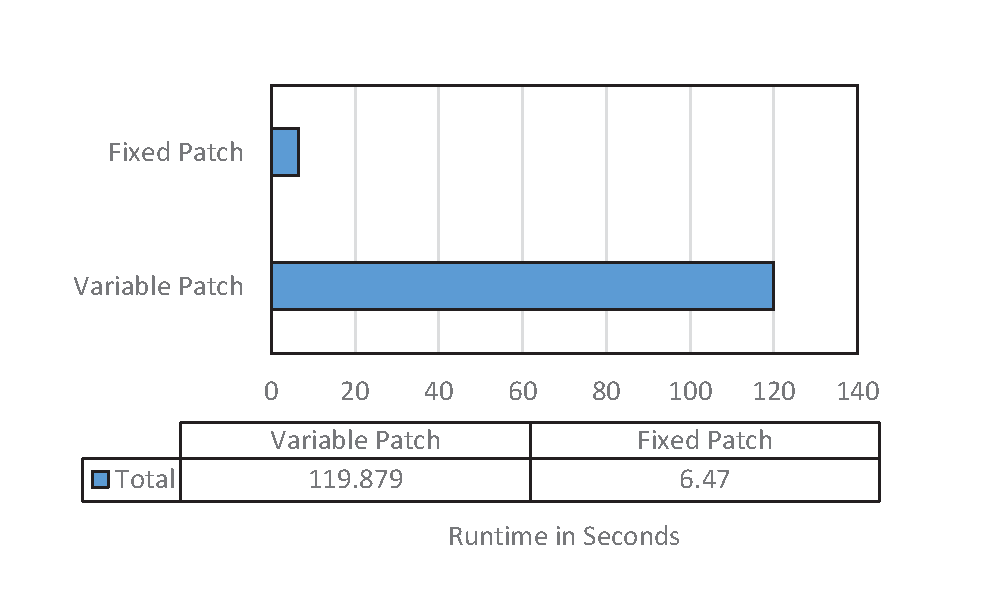
\includegraphics[width=.45\textwidth]{figures/patch_result_single.eps}
\caption{Time taken to perform patch extraction and averaging for fixed versus variable patch locations on a single machine}
\label{fig:patch_result}
\end{figure}

We show the time taken to extract 100x100 patches from 7 images sized 1920x1080 in SciDB. Surprisingly, even though fixed patch extraction can be done as a single nested SciDB query, iterating and slicing out individual image planes from the image volume and then assembling the patch volume is significantly faster on a single node. We will revisit this experiment on the cluster in \S \ref{sec:clusterexp}.

\subsubsection{Convolution}

\begin{figure}[h]
\centering
\includegraphics[width=.55\textwidth]{figures/convo_single.eps}
\caption{Performance of \texttt{window()} operation in SciDB versus an Image convolution operation in Native C code.}
\label{fig:convo_result}
\end{figure}

We compare the performance of SciDB's windowed aggregation function when compared to a hand-written image convolution function in C (Figure \ref{fig:convo_result}). SciDB is once again over an order of magnitude slower than Native C code implementations of Image processing, for which the exact reasons not fully understood. We will continue our experiments on a much larger set of machines in S \ref{sec:clusterexp}

\subsection{Cluster-Based Experiments}
In this section, we present the results of running our image processing operations on a much larger cluster of 16 nodes on AWS, using the cluster setup explained in \S \ref{sec:eval}. We begin with a comparison of each of the benchmarks against the MPI baselines, and then proceed to show a breakdown of the runtime in \S\ref{sec:breakdown}.

\subsubsection{Image Load Times}

\begin{figure}[h]
\centering
\includegraphics[width=.50\textwidth]{figures/image_load.eps}
\caption{Time taken to convert and load the image dataset from files on the shared NFS mount into raw pixel values in a 16-node SciDB Cluster }
\label{fig:image_load}
\end{figure}

A non-trivial portion of time was devoted to the actual loading and conversion of the compressed JPG data into the raw pixel values loaded into the image volume. Figure \ref{fig:image_load} shows the time taken to load 10,100 and 1000 images respectively on the 16 node cluster. It should be noted that the 10, 100 and 1000 images are roughly 0.474, 4.74 and 47.4 GB respectively. 


\subsubsection{Comparison with MPI}\label{sec:clusterexp}
In this section, we compare the runtime of the image processing operations in SciDB against their MPI counterparts. 

\begin{figure*}[htp]
\centering
	\subfigure[WIA]{\label{fig:wia}\includegraphics[width=0.45\textwidth]{figures/wia.eps}} \hspace{1 em}
    \subfigure[IPE]{\label{fig:ipe}\includegraphics[width=0.4\textwidth]{figures/ipe.eps}}
	\subfigure[CONV]{\label{fig:conv}\includegraphics[width=0.5\textwidth]{figures/convo.eps}} \hspace{1 em}
    \subfigure[APNN]{\label{fig:apnn}\includegraphics[width=0.85\textwidth]{figures/apnn.eps}}
	\caption{Performance of Image Operations in SciDB versus the Baseline MPI Versions. All run-times are the average of 3 runs, with variation being within \~2\% of the actual runtime. APNN benchmarks for larger datasets did not finish running even after 6 hours.}
	\label{fig:mpi_result}
\end{figure*}

\textbf{Weighted Image Average}: In Figure \ref{fig:wia}, we see the runtime of SciDB for the WIA benchmark for 10, 100 and 1000 images on the 16 node cluster. The MPI version of this operation is roughly between $21\times$ to $91\times$ faster than the SciDB counterpart for the same operation.

\textbf{Image Patch Extraction}: Contrary to our experiences with the IPE benchmark in a single node, Figure \ref{fig:ipe0}, shows a slowdown in the performance of IPE when using a variable patch rather than a fixed patch from a volume of images.


\begin{figure}[h]
\centering
\includegraphics[width=.50\textwidth]{figures/patch_result_cluster.eps}
\caption{Fixed vs. Variable patch extraction on the 16 node cluster.}
\label{fig:ipe0}
\end{figure}


In Figure \ref{fig:ipe}, we see the runtime of SciDB for the IPE benchmark (fixed patches) when varying the dataset size. Unlike the WIA benchmark, where the entire image volume was flattened to a single image, the IPE benchmark shows significant improvement in runtime and is within an order of magnitude in terms of performance when compared to the baseline MPI version, as the $100\times100$ image patch extraction and averaging of a 1000 1080p images is only $\sim 2.14\times$ slower than its corresponding MPI version.

\textbf{Convolution} In Figure \ref{fig:conv}, we compare the performance of the MPI baseline that performs convolution on a set of images against the SciDB \texttt{window()} function, which performs the equivalent operation. Again, SciDB is an order of magnitude slower than the MPI implementation across the board.

\textbf{All Pairs Nearest Neighbors}: For the APNN benchmark, we perform the APNN step with an additional set of images: 10, 100 and 1000 64x64 thumbnails (Figure \ref{fig:apnn}. The missing data-points indicate SciDB failing to finish execution even after ~6 hours of runtime. 


\subsubsection{Timing Breakdown and Analysis}\label{sec:breakdown}
We now provide the timing breakdown for two of the operations of interest, the WIA and APNN benchmarks in Figure \ref{fig:breakdown}. We can see from the figures that the runtime for these queries is dominated by the cross join query, more so for APNN.

\begin{figure*}[htp]
\centering
	\subfigure[WIA]{\label{fig:wiabreak}\includegraphics[width=0.50\textwidth]{figures/wia_breakdown.eps}} \hspace{1 em}
    \subfigure[APNN]{\label{fig:apnnbreak}\includegraphics[width=0.45\textwidth]{figures/apnn_breakdown.eps}}
	\caption{Performance of Image Operations in SciDB versus the Baseline MPI Versions. All run-times are the average of 3 runs, with variation being within \~2\% of the actual runtime. APNN benchmarks for larger datasets did not finish running even after 6 hours.}
	\label{fig:breakdown}
\end{figure*}

\section{Conclusions and Future Work}\label{sec:future}
In this work, we have implemented a number of image processing operations in SciDB and compared its performance against a simple MPI implementation. SciDB is many orders of magnitude slower than the corresponding MPI implementation and we conjecture the following reasons that contribute towards the slow performance of SciDB:

\begin{itemize}
\item SciDB stores raw pixel values and is unable to take advantage of domain-specific image compression schemes such as JPEG. This leads to a rapid expansion of the number of images stored which, in turn leads to massive I/O traffic during loading and execution of operations in SciDB.
\item Except for Convolution, all of the image processing operations studied require some kind of cross-join operation, with APNN requiring a cross-join across the image dimension, leading to massive increase in the amount of data to be materialized. 
\end{itemize} 

The idea of SciDB or other array databases to perform image processing is interesting as it allows for these operations to be expressed in the form of queries. However, given the lack of support for domain-specific compression formats and the extremely slow execution times, we believe there a lot of work to do before SciDB becomes a viable platform for image and video processing. 

\section{Code Availability}

All of the code presented in this report is available here:

{\tt \small
\begin{verbatim}
 http://github.com/suhailrehman/scidb-image
\end{verbatim}
}

The custom cluster launch scripts are also made available here:

{\tt \small
\begin{verbatim}
 http://github.com/suhailrehman/scidb-starcluster
\end{verbatim}
}


{\footnotesize 
\bibliography{template}
}
\end{document}







